\chapter{Background}
\label{sec:background}
	This work addresses several fields within Computer Vision/Machine Learning research. Chapter 2 explores these areas and builds up a solid basis to carry out further research. The chapter also contains background information for readers who come from other fields.
	
	\autoref{sec:bg:object_detection} describes Object Detection. The field is concerned with finding and classifying objects within images. \autoref{sec:bg:training} investigates methods to train models when limited data is available. \autoref{sec:bg:speed_optimization} illustrates work about increasing the inference speed of computer vision methods. \autoref{sec:bg:related_work} describes related work in the application of gate detection for autonomous drone racing.
	\section{Object Detection}
	Object Detection is a well studied topic since the very beginning of computer vision. It can be separated in two individual problems which are classification: Which object does the image contain? and localization: Where in the image is the object?.
	
	Existing methods can broadly be grouped in three categories. These are described in the following:

	\subsubsection{Shallow Methods}
	
	Usually filters are handcrafted or learned separately. Their response is fed into a classifier. The detector pipeline is applied on the image in sliding window fashion. The results are filtered by a final non-maximum suppression stage. 
	
	Popular features are haar-features \cite{Viola2004} and the Histogram of Gradients\cite{Forsyth}. These methods give good results as long as the object is fully visible and the position in the test set does not change too much. This issue gave raise to deformable part models where parts of the object are modeled individually and connected with mathematical springs \cite{Viola2004}.
	
	The methods are usually pretty fast but not so accurate.
	
	\subsubsection{Two Stage Detectors}
	
			\paragraph{Scalable Object Detection using Deep Neural Networks\cite{Erhan}}
			\begin{itemize}
				\item[-] Generates number of bounding boxes as object candidates (class agnostic) and confidences for each box
				\item[-] For each Bounding Box a classifier is run e.g. DNN
				\item[-] Training: If the number of boxes k is larger than the number of objects b, only b boxes are matched while the confidence of the others is minimized
				\item[-] Assignment problem $$F_{match}(x,l) = \frac{1}{2}\sum_{i,j}x_{ij}||l_i - g_j||^2_2$$ where $x_ij$ is one if the ith prediction is assigned to the jth ground truth object
				\item[-] Confidence: 
				$$F_{conf}(x,c) = - \sum_{i,j}x_{ij}*\log(c_i)-\sum_{i}(1-\sum_{j}x_{ij})\log{1-c_j}$$
				\item[-] Speed up training by clustering (kmeans) of ground truth and using it as prior (prior matching)
				\item[-] Can be defined to output boxes only for a particular class by training the bounding boxes on that class
				\item[-] Number of parameters grows linearly with number of classes
				\item[-] Authors argue two step process (region proposal + classification) is better
				\item[-] Architecture based on AlexNet
				\item[-] Predicted boxes are merged using non-maxima surpression
				\item[-] One shot(50\%), +2scales (75\%)
				\item[-] OverFeat/ Selective Search are faster but much more expensive
			\end{itemize}
			
	
	Methods consist usually of two stages.An example is R-CNN\cite{Ren}. 
	\begin{itemize}
		\item Object Proposal: A convolutional net proposes regions that contain an object. This is either done in sliding window fashion or in one pass.
		\item Classification: All proposed regions are fed into a classifier. This can either be a "traditional" one or another CNN.
	\end{itemize}
	These methods are usually pretty accurate but also slow.
	\subsubsection{One Stage Detectors}
	
	\begin{figure}[h]
		\centering
		\begin{minipage}{0.4\textwidth}
			\centering
			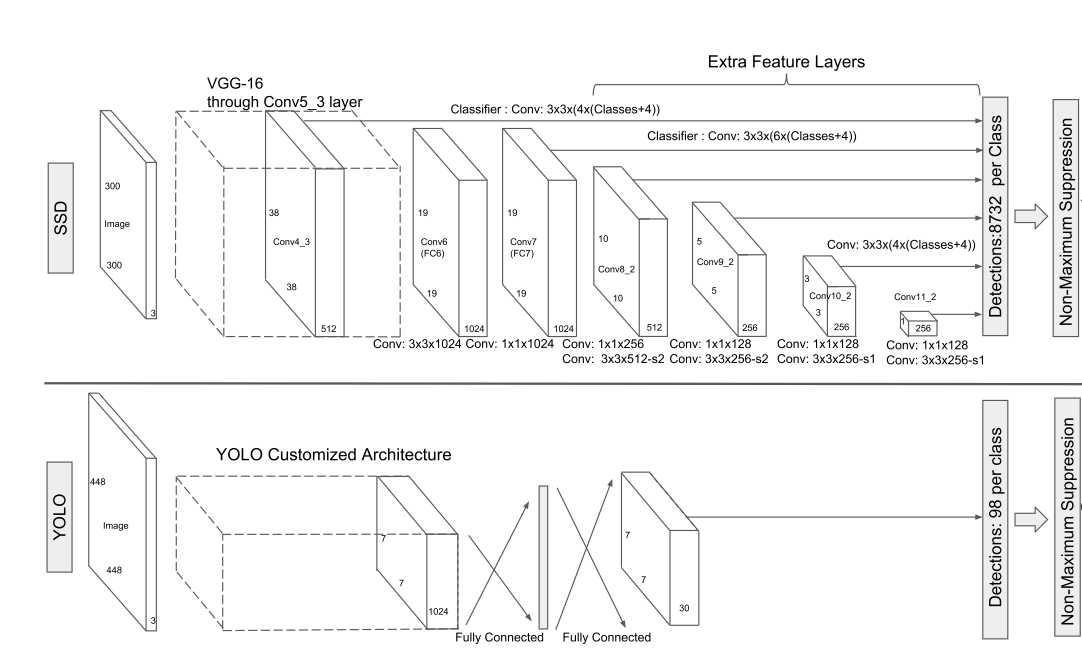
\includegraphics[height=2.5cm]{fig/architecture}
			\caption{Typical Architecture for One Stage Detectors}
			\label{fig:architecture}
		\end{minipage}
		\hspace{2cm}
		\begin{minipage}{0.4\textwidth}
			\centering
			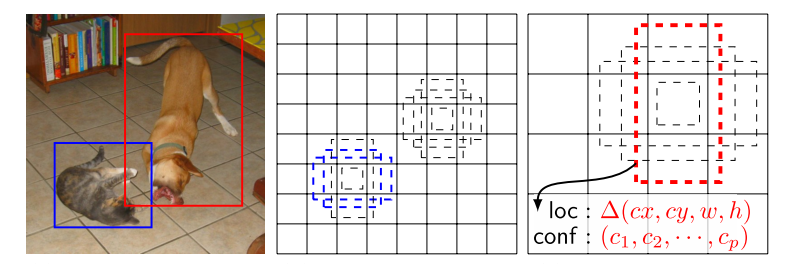
\includegraphics[height=2.5cm]{fig/anchors}
			\caption{Example of \cite{Liu}, the GT box of the cat is matched to two anchor boxes which get responsible for predicting that box. The GT box of the dog is matched to one anchor box.}
			\label{fig:anchors}
		\end{minipage}
	\end{figure}
	
	Most current methods rely on the same principle as Yolo/SSD: A convolutional regression layer is stacked on top of a "base network" that has been trained for image classification e.g. VGG-16. The output layer evaluates feature map(s) of the base network and predicts class confidences, and coordinate offsets for a predetermined set of bounding boxes (so called "prior boxes", "anchor boxes" or "default boxes"). The predictions are filtered in a final non-max-suppression step. During training one has to determine which anchor box is responsible for predicting a certain object. This "matching strategy" differs from method to method but is usually based on the intersection-over-union between the ground truth box and anchor box. \autoref{fig:anchors} illustrates the concept. The final loss function calculates the difference between the responsible boxes and the ground truth. 
	
	Within this framework several approaches exist that either change the base network or modify layers in between: \cite{ChengchengNing2017} propose to include an inception module in the network architecture to reduce computation while keeping/increasing performance. They also propose a more efficient non-max-suppression method. \cite{Wu} uses \textit{SqueezeNet} as base network and a mixture between the ssd and yolo loss function as training goal. \cite{Xiang} investigates the receptive fields of SSD and tries to incorporate more context, especially on lower feature maps, to increase detection rate for small objects.\cite{Linb} applies the framework for vehicle detection. They use \textit{GoogLeNet} as base network (and investigate several others).\cite{TripathiSanDiego} apply a network very similar to YoloV2 and investigate 8bit quantization of the model to make it runnable on embedded devices.
	
	A common problem of one stage detectors is the imbalance between background and object samples. Most methods upweigh the positive samples and/or use hard negative mining. \cite{Lin} introduces the \textit{Focal Loss} which focuses on sparse positive samples by design.
	
	\subsubsection{LCDNet\cite{TripathiSanDiego}}
	
	Aims to bring one shot detection to be runnable on embedded devices.
	
	\begin{itemize}
		\item Quantizies model for inference with 8bit. Records min and max value for each layer and quantizes everything between 0,255
		\item Replaces fully connected layers with convolutional layers
		\item Replaces LeakyRelu with Relu in all but the last (faster?)
		\item Softmax on classification, Sigmoid on confidence
		\item Sigmoid if only one class
		\item quantization mainly effects localization
	\end{itemize}
	
	\subsection{\cite{Linb}}
	
	\begin{itemize}
		\item Uses GoogLeNet as base network
		\item investigates image augmentation and hard negative mining
		\item Uses confidence score plus class probability although only one object shall be detected
	\end{itemize}
		

\begin{table}[]
	
	\caption{Object Detection}
	\label{my-label}
	\begin{tabular}{|p{3cm}|p{3cm}|p{3cm}|p{3cm}|p{3cm}|p{3cm}|p{3cm}|p{3cm}|}
		\hline
		& \multicolumn{3}{l|}{Traditional} & \multicolumn{4}{l|}{Deep}   \\ \hline
		& Viola\&Jones    				   & HoG    & DPM   		   & R-CNN    & YOLO         & SSD & OverFeat \\ \hline
		Feature Detector & Haar					   & HoG    & Multiple Hogs and virtual springs   & Learned by CNN     &  Learned by CNN            & & \\ \hline
		Detection & \multicolumn{3}{l|}{Sliding Window, high filter responses indicate there is an object} & NN in sliding window detects regions for possible objects, For each proposed region a classification is run & Image is split in Grid each Grid spawns Bounding boxes and gives class probabilities & & \\
		\hline
		Accuracy (voc) &  & & & 73.2 mAP & 63.4 mAP & 74.3 mAP & \\ 
		\hline
		Speed & & & & 7 FPS (Faster-RCNN) & 45 FPS & 59 FPS & \\
		\hline
		Strengths & & & & & &  &\\
		\hline
		Weaknesses & & & & & &  &\\
		\hline
		\end{tabular}
		
		\end{table}



%\section{Pose Estimation}
\label{sec:pose_estimation}
	\subsection{(Re-) Localization}
	\paragraph{PoseNet: A Convolutional Network for Real-Time 6-DOF Camera Relocalization \cite{Kendall}}
	\begin{itemize}
		\item[-] Relocalizes, is trained on images from the scenes where it is applied	\item[-] Accuracy 2m and 3$\degree$  in 50 km$^2$ outdoors, 0.5m and 5$\degree$ indoors, 5ms per frame
		\item[-] ConvNet 23 layers, Image resolution 224x224
		\item[-] transfer learning from recognition/classification datasets (ConvNet is trained on classification tasks)
		\item[-] based on GoogleNet, affine regressors instead of softmax\item[-] automatic training data generation (structure from motion)
		\item[-] learns p from arbitrary global reference frame
		\item[-] $loss(I) = || \hat{x}-x||_2 + \beta*||\hat{q}-\frac{q}{||q||}||_2$
		\item[-] separating position/orientation led to drop in performance
		\item[-] PoseNet evaluation at single center crop + Dense PoseNet 128 uniformly spaced crops (time increase 95ms, only slight accuracy increase)
		\item[-] Training data generated using structure from motion (Cambridge Scene) and 7 Scenes (Microsoft) for indoor
		
	\end{itemize}
	\paragraph{A Deep Learning Based 6 Degree-of-Freedom
		Localization Method for Endoscopic Capsule Robots \cite{Turan2017}}
	\begin{itemize}
		\item[-] not published yet?
		\item[-] Uses 6-DOF camera pose directly
		\item[-] based on GoogleNet (9 Inception modules) trained on ImageNet
		\item[-] $loss(I) = ||\hat{x}-x||_2 + ||\hat{q}-q||_2$
		\item[-] Dataset of 10 000 frames taken from LM103 - EDG (EsophagoGastroDuodenoscopy) Simulator
		\item[-] 0.18cm RMSE on a trajectory of 18cm
		\item[-] Although 3 different cameras are used and the frames are separated for training and testing, its still the same "stomach". With 10 000 frames on a trajectory of 18 cm, won't the system just recognize the position?
		\item[-] Ground truth determined by seperate cameras 
	\end{itemize}
	\subsubsection{Object Pose Estimation}
	\paragraph{3D generic object categorization localization and pose estimation \cite{Savarese}}
	\begin{itemize}
		\item[-] Other approaches use different class for different poses
		\item[-] Object model is separated in different parts of the object based on different view points (front view)
		\item[-] Different parts are connected when another part is visible from the front view via affine transformation
		\item[-] Generally such models can't handle inter class variations very good or increase in complexity as number of parts is increased. In this paper this is apparently not the case
	\end{itemize}
	\paragraph{Uncertainty-Driven 6D Pose Estimation of Objects and Scenes from a Single RGB Image
		Eric \cite{Brachmann}}
	\begin{itemize}
		\item[-] Intermediate representation are object coordinates, continious part labeling that are jointly regressed for every pixel in the image
		\item[-] Based on auto context (Classifiers with several stages)
		\item[-] (1) (Auto context) Random forest with L1 regularization predicts labels and object coordinates for every pixel (2) Ransac predicts poses from 2d-3d correspondences guided by uncertainty labels
		(3) Refinement
		\item[-] Random forest predicts (probability to belong to object + 3d coordinate|given belonging to object)
		\item[-] Stacked Forests (Auto context) refine output on previous smoothed output (Geodesic Forest). The smoothing is done to enforce coupling of neighbors 
		\item[-] RANSAC formulates hypothesis by drawing 4 correspondences and solving PnP
		\item[-] Outperforms PoseNet in indoor localization
		\item[-] 6D within 5cm and 5 degree only 40 \% (With RGB-D 82.5\%), on other set 50 \% with unknown scene average median error 8.5cm 3.3°
		\item[-] Biggest translational error in z direction
		\item[-] Multi object detection/pose estimation in 1-4 seconds, not optimized, most time spend in searching for object hypothesis
	\end{itemize}
	\paragraph{A Comparative Analysis and Study of Multiview CNN Models for Joint Object Categorization and Pose Estimation\cite{Elhoseiny}}
	\begin{itemize}
		\item[-] While detection needs pose invariant features, pose estimation needs the pose
		\item[-] Single instance 3d model
		\item[-] Discrete pose approaches (pose as classification)
		\item[-] Trains pose regressor and classifier on output of different levels to measure quality of features
		\item[-] Later layers "forget" about pose, paper suggests early branching
	\end{itemize}
	\subsection{Other}
	\paragraph{Deformable Convolutional Networks \cite{Dai}}
	\begin{itemize}
		\item[-] Addresses problem of modeling geometric transformations
		\item[-] Introduces \textit{Deformable Convolution} which adds 2D offsets to the regular sampling grid. The offsets are learned from the data.
		\item[-] Introduces \textit{Deformable RoI pooling} which adds offsets to bins of pooling layers. The offsets are also learned from the data.
		\item[-] Further alternatives to have more variable feature maps: Spatial Transformer Networks, Active Convolution, Effective Receptive Field, Atrous Convolution, DeepID-Net, Spatial manipulation in RoI pooling (handcrafted), DPM (handcrafted)
		\item[-] Light-weight version of STN, easier to train and to integrate
		\item[-] Receptive fields seem to scale with the size of objects
		\item[-] Model complexity is increased by only 1-2%
	\end{itemize}
	

\newpage
\section{Training}
\label{sec:bg:training}

The performance of machine learning models heavily depends on the available training data. If the labelled examples do not sufficiently represent the real world, any learned algorithm will fail when applied in the wild. As the model complexity increases, its potential performance increases as long as there is enough training data available with which the model parameters can be tuned. Is not enough training data available the model may overfit to the training data, meaning it will perform well on the training set but fail on any other data set. Overfitting can be introduced by a limited amount of available training samples but also when the training data stems from a different domain than the test data. This scenario is also referred to as domain shift.

For the computer vision system investigated in this work this mean

If there are not enough labelled samples models can overfit to the particular training set. This means a low error can be achieved on the training data but the model performs poorly when applied in the wild.

Similar effec
\newpage
\section{Speed Optimization}
\label{sec:bg:speed_optimization}

\todo{What is we want to minimize? Nr. of computations + Memory usage}

LCD NET
\newpage
\section{Related Work}
IROS2018 is not the first edition of autonomous drone racing. This section describes related work in the field of gate detection for autonomous drone racing.